\chapter{Memory architecture and data locality}
\begin{center}
    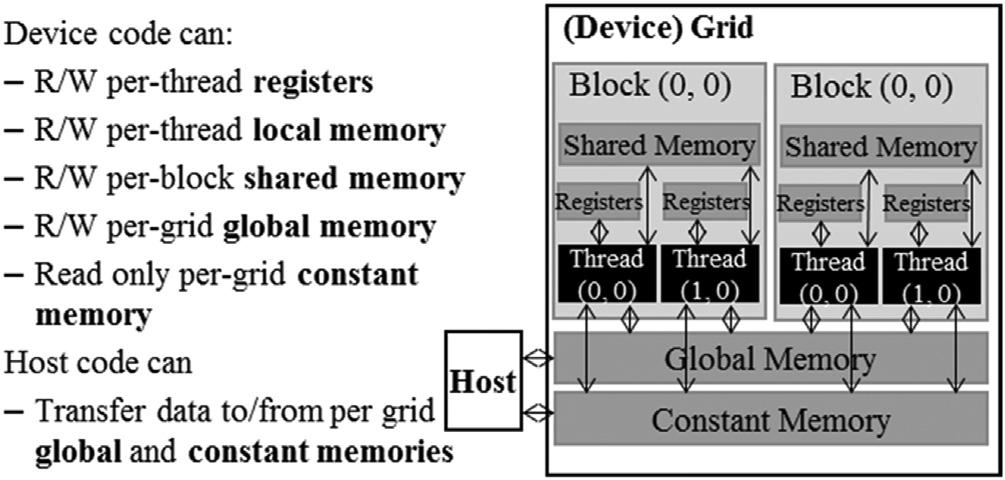
\includegraphics[width=0.8\linewidth]{Images/Memories/memory_types.png}
\end{center}
\begin{itemize}
    \item \textbf{Global memory}:
          \begin{itemize}
              \item Can be both read and written by \textsl{Device}.
              \item Can be both read and written by \textsl{Host}.
          \end{itemize}
    \item \textbf{Constant memory}:
          \begin{itemize}
              \item Offers short-latency high-bandwidth \textbf{\textsl{read-only access}} to \textsl{Device}.
              \item Can be both read and written by \textsl{Host}.
          \end{itemize}
    \item \textbf{Local memory}:
          \begin{itemize}
              \item Resides in the global memory, but is not shared across threads. Each thread has its own private local memory, where places the data that is private to the thread but cannot be allocated in the registers. This data includes statically allocated arrays, spilled registers, and other elements of the thread’s call stack.
          \end{itemize}
    \item  \textbf{Registers and Shared memory}:
          \begin{itemize}
              \item Are on-chip memories. Variables that reside in registers/shared memory can be accessed at very high speed in highly parallel manner.
              \item Registers are allocated to individual threads; each thread can access its own set of registers.
              \item \textsl{Kernel function typically uses registers} to store frequently accessed variables that are private to each thread.
              \item \textsl{Shared memory is allocated to thread blocks}; all threads in a block can access shared memory variables declared for the block.
                    \begin{itemize}
                        \item Shared memory is an efficient means by which threads can cooperate by sharing their input data and intermediate results.
                        \item By declaring a CUDA variable in one of the CUDA memory types, a CUDA programmer dictates the visibility
                              and access speed of the variable.
                    \end{itemize}
          \end{itemize}
\end{itemize}

\begin{tcolorbox}
    \subsubsection{CPU vs GPU Register architecture}
    \begin{itemize}
        \item When CPUs context switch between different threads, they save the registers of the outgoing thread to memory and restore the registers of the incoming thread from memory.
        \item In contrast, GPUs achieve zero-overhead scheduling by keeping the registers of all the threads that are scheduled on the processing block in the processing block’s register file.
        \item This way, switching between warps of threads is instantaneous because the registers of the incoming threads are already in the register file. Consequently, GPU register files need to be substantially larger than CPU register files
    \end{itemize}
\end{tcolorbox}
\section{- Advantages of Registers over Global Memory}
\begin{itemize}
    \item Global memory is implemented with DRAM technology, implying long access latencies and relatively low access bandwidths.
    \item The registers on the other hand, are on the processor chip, which implies very short access latency and very large access bandwidth, compared to the global memory.
          \begin{itemize}
              \item Floating-point addition with operands on global memory:
                    \begin{center}
                        \texttt{load r2, r4, offset}\\
                        \texttt{fadd r1, r2, r3}
                    \end{center}
                    \texttt{load} instruction adds an offset value to the contents of \texttt{r4} to form an address for the operand value. It then accesses the global memory and places the value into register \texttt{r2}. Once the operand value is in \texttt{r2}, the \texttt{fadd} instruction performs the floating-point addition using the values in \texttt{r2} and \texttt{r3} and places the result into \texttt{r1}.\\
                    Since the processor can fetch and execute only a limited number of instructions per clock cycle, the version with an additional load will likely take more time to process than the one without.
          \end{itemize}
    \item Whenever a variable is stored in a register, its accesses no longer consume off-chip global memory bandwidth. \textsl{A subtler point is that each access to registers involves fewer instructions than access to the global memory.}
          \begin{itemize}
              \item Floating-point addition with operands on built-in registers:
                    \begin{center}
                        \texttt{fadd r1, r2, r3}
                    \end{center}
                    The register files \texttt{r2} and \texttt{r3} are the files where input values can be found. The addition of \texttt{r2} and \texttt{r3} are stored in \texttt{r1}.
          \end{itemize}
    \item In modern computers the energy that is consumed for accessing a value from the register file is at least an order of magnitude lower than for accessing a valuefrom the global memory. Accessing a value from registers has a tremendous advantage
          in energy efficiency over accessing the value from the global memory.
\end{itemize}

\section{Shared memory vs Registers}
\begin{center}
    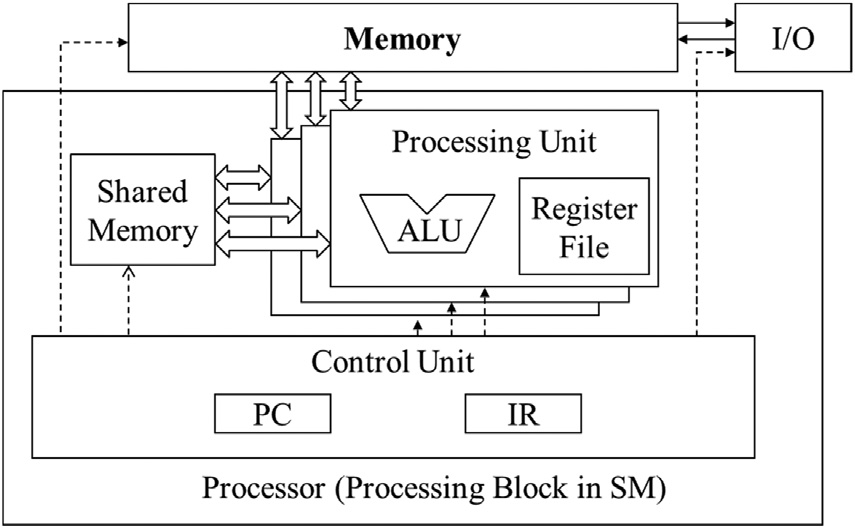
\includegraphics[width=0.5\linewidth]{Images/Memories/CUDA_device_SM.png}
\end{center}
\begin{itemize}
    \item Shared memory
          \begin{itemize}
              \item Is designed as part of the memory space that resides on the processor chip.
              \item When the processor needs to access the data, it still has to perform the \texttt{load} operation same as when accessing the data from the global memory.
              \item However, as the shared memory resides on-chip, it can be accessed with much lower latency and much higher throughput than in global memory access.
              \item Because of the need to perform a load operation, shared memory has longer latency and lower bandwidth than registers.
              \item In computer architecture terminology the shared memory is a form of \textsl{scratchpad memory}.
          \end{itemize}
    \item One important difference between \textsl{Shared Memory} and the \textsl{Registers} is that, \textsl{Shared Memory is accessible by all the threads in a block}. This is contrary to the \textsl{register data, which is private to a thread}.
    \item CUDA device SM typically employs multiple processing units to allow multiple threads to make simultaneous progress.
    \item Threads in a block can be spread across these processing units.
    \item Therefore, the hardware implementations of the shared memory in these CUDA devices are typically designed to allow multiple processing units to simultaneously access its contents to support efficient data sharing among threads in a block.
\end{itemize}

\section{- Declaring program variables into the various memory types}
\begin{center}
    \begin{tabular}{c|c|c|c}
        Variable declaration                          & Memory   & Scope    & Lifetime    \\
        \hline
        Automatic variables other than arrays         & Register & Register & Grid        \\
        Automatic array variables                     & Local    & Local    & Grid        \\
        \_\_device\_\_ \_\_shared\_\_ int SharedVar;  & Shared   & Shared   & Grid        \\
        \_\_device\_\_ int GlobalVar;                 & Global   & Global   & Application \\
        \_\_device\_\_ \_\_constant\_\_ int ConstVar; & Constan  & Constan  & Application \\
    \end{tabular}
\end{center}
\begin{itemize}
    \item If a variable’s scope is a single thread, a private version of the variable will be created for every thread; each thread can access only its private version of the variable.
    \item Lifetime tells the portion of the program’s execution duration when the variable is available for use: either within a grid’s execution or throughout the entire application.
    \item If a \textbf{variable’s lifetime is within a grid’s execution, it must be declared within the kernel function body and will be available for use only by the kernel’s code}. If the kernel is invoked several times, the value of the variable is not maintained across these invocations. Each invocation must initialize the variable in order to use it.
    \item If a variable’s lifetime is throughout the entire application, it must be declared outside of any function body. The contents of these variables are maintained throughout the execution of the application and available to all kernels.
    \item Variables that are not arrays are \textsl{scalar} variables. \textbf{All automatic scalar variables that are declared in kernel and device functions are placed into registers.} The scopes of these automatic variables are within individual threads. When a \textbf{kernel function declares an automatic variable, a private copy of that variable is generated for every thread that executes the kernel function. When a thread terminates, all its automatic variables cease to exist.}
\end{itemize}